\providecommand{\main}{..}		% Override relative path to the main file (already set in main file)
\documentclass[../InterneDSLs.tex]{subfiles}
\begin{document}

\chapter{Bau des Prototypen}\label{SEC:Prototype}

\section{Aufbau}
Die Verarbeitung der Grammatik erfolgt nach dem folgenden Schema:
\begin{itemize}
	\item Parsen der Grammatik
	\item Aufbau des Syntax-Baumes
	\item Abbildung in einen Graphen, der die Aufrufreihenfolge abbildet
	\item Generierung der Interfaces mit StringTemplates
\end{itemize}

\section{Parsen der Grammatik}
Für das Parsen der Grammatik wurde ANTLR4 verwendet, der adaptive LL(*)-Parser generieren kann, die Grammatiken zur Laufzeit analysieren können, statt zur Compilezeit (siehe~\cite[S. xiii ff]{Parr.2012}). ANTLR selbst ist in Java geschrieben und kann Parser für verschiedene Zielsprachen generieren (u.a. Java, C++, C\#, Python, vgl.~\cite{antlrcodegeneration.github}). Da neue Features vorrangig für den Parser in Java entwickelt werden, und da als Zielsprachen JVM-Sprachen ins Auge gefasst wurden, wird auf dem Parser in Java aufgebaut werden.

Um die Grammatiken zu notieren verwendet ANTLR eine Syntax die sich nicht an der ISO-Norm sondern an einer alten EBNF-Variante orientiert. In dieser Syntax wurde eine Grammatik erstellt, um die in Abschnitt~\ref{SEC:SetSyntax} festgelegte Notation der EBNF zu parsen (Listing~\ref{LST:EBNFGrammar}). Der Hauptgrund zum Erstellen einer neuen Syntax für Grammatiken, statt die von ANTLR zu verwenden, ist der, dass die Mächtigkeit von ANTLR für den Anwendungsfall nicht benötigt wird; es werden verschiedene Optionen, Importe, Token und Aktionen bereitgestellt~\cite[S. 265ff]{Parr.2012}, mit denen man den von ANTLR generierten Code beeinflussen kann. Die notwendigen Optionen werden beim Aufruf vom Prototypen selbst angegeben.

Beim verfassen der Grammatik wurde schon darauf Rücksicht genommen, dass man Schlüsselworte und Typen (einer Programmiersprache) angeben kann (siehe Listing~\ref{LST:EBNFGrammar} Zeile 24-33).

\subsection{Festgelegte Syntax}\label{SEC:SetSyntax}
Die abstrakte Syntax entspricht der der EBNF mit Sequenzen, Gruppierungen, optionalen Elementen und Wiederholungen. Die konkrete Syntax bzw. Notation der EBNF richtet sich an der ISO-Norm orientiert (\cite[S. 7]{scowen1996international}),sich aber leicht davon (Tabelle~\ref{TAB:EBNFSyntax}). So gibt es in der Sequenz keine Trennzeichen (im ISO-Standard das Komma) und es werden keine Kommentare und keine Ausnahmen unterstützt. Die Nicht-Terminal werden, wie in der BNF~\cite[S. 3]{crocker1997augmented}, in spitzen Klammern notiert um sie von Schlüsselworten und Typen zu unterscheiden (siehe Listing~\ref{LST:EBNFGrammar}, Zeilen 28-33). In Listing~\ref{LST:EbnfNumbers} wurde eine Grammatik für ganze Zahlen definiert, um die Notation an einem gängigen Beispiel zu zeigen.

\begin{table}[ht]
\centering
\begin{tabular}{l|c}
\textbf{Konstrukt}     & \textbf{Syntax}\\\hline
Definition             & \verb|=|\\
Alternative            & |\\
Regel-Endzeichen       & \verb|;|\\
Gruppierung            & \verb|( ... )|\\
Optionales Element     & \verb|[ ... ]|\\
Optionale Wiederholung & \verb|{ ... }|\\
Nicht-Terminal         & \verb|< ... >|\\
\end{tabular}
\caption{EBNF-Syntax-Elemente}
\label{TAB:EBNFSyntax}
\end{table}

\begin{lstlisting}[caption={Zahlen in der festgelegten Notation},label={LST:EbnfNumbers}]
<digitNotZero>    = '1' | '2' | '3' | '4' | '5' | '6' | '7' | '8' | '9' ;
<digit>           = '0' | <digitNotZero> ;
<naturalNumber> = <digitNotZero> { <digit> } ;
<integer>         = '0' | [ '-' ] naturalNumber ;
\end{lstlisting}

\begin{figure}[ht]
\lstinputlisting[linerange={3-35},caption={EBNF-Grammatik (Auszug)},label={LST:EBNFGrammar}]{Bnf.g4}
\end{figure}

\subsection{Traversieren des Parse-Trees}
Um den Parse-Tree der eingelesenen Grammatik zu verarbeiten gibt es bei ANTLR4 zwei Möglichkeiten: entweder können die generierten Listener oder Visitor überschreiben werden(vgl.~\cite[S. 112 ff]{Parr.2012}). Die Visitors sollte man implementieren, falls man größtmögliche Kontrolle über das traversieren des Baumes benötigt. Da das aber nicht nötig ist, werden hier nur die Listener erweitert, um aus den EBNF-Konstrukten (die praktisch Strings entprechen) einen Baum aus eigenen Klassen generiert. Dadurch wird eine Typ-Sicherheit hergestellt, die durch die Strings im EBNF-Parser selbst nicht gegeben ist.

Abbildung~\ref{FIG:TypesBNF} zeigt die eigenen Typen des Baumes, der dem Parse-Tree entspricht; in ihm finden sich die Konstrukte der EBNF wieder (z.B. Regeln, Sequenzen, Alternativen, vgl. Abbildung~\ref{LST:EBNFGrammar}). Aus dem Baum dieser Typen werden die Interfaces generiert, wie im folgenden Abschnitt~\ref{SEC:EBNFtoInterface} erklärt wird.

\begin{figure}[ht]
\centering
\includegraphics[width=\linewidth]{\main/10_Pictures/BNF-Types}
\caption{Typen des BNF-Baumes}
\label{FIG:TypesBNF}
\end{figure}

\section{Abbildung von EBNF auf Interfaces}\label{SEC:EBNFtoInterface}
Aus dem Baum ein Graph generiert, dessen Abfolge von Knoten und Kanten die Konstrukte der EBNF darstellt. Die Knoten werden dabei dazu verwendet, die Scopes für das Object Scoping zu repräsentieren, der Typ und die Anzahl der Kanten repräsentierten die Konstrukte der EBNF selbt. Wie die Konstrukte genau abgebildet werden, wird in den folgenden Abschnitten erklärt. Neben den trivialen Fällen wird auf einige verschachtelte Konstrukte eingegangen um zu zeigen, dass einige Konstrukte im Graph verwendet werden, die aus den trivialen Fällen nicht ersichtlich sind.

Da bei mehreren Schleifen in einer Alternative von mehreren Interfaces geerbt werden muss, kommen abstrakte Klassen nicht infrage, da diese nur von einer anderen Klasse erben können. Interfaces können stattdessen mehrere andere erweitern.

Zuerst werden jedoch die Eigenschaften des Graphen erläutert und dazu eine entsprechende Bibliothek ausgewählt.

\subsection{Eigenschaften des Graphen}
Aus der Struktur der EBNF gehen verschiedene Eigenschaften des Graphen heraus; er Graph ist
\begin{itemize}
	\item gerichtet (wegen der Sequenz),
	\item zyklisch (Wiederholung),
	\item ungewichtet (keine Alternative wird bevorzugt) und
	\item kann parallele Kanten enthalten (Alternative).
\end{itemize}
Diese Eigenschaften bezeichnen einen gerichteten, zyklischen Multi- bzw. Pseudograph. Die parallelen Kanten haben eine eigene Identität (Name und Typ), mit der man sie von anderen Kanten mit dem selben Quell- und Zielknoten unterscheiden kann.

Da es bei allen im folgenden vorgestellten Abbildungen jeweils einen Knoten ohne eingehende Kanten und einen Knoten ohne ausgehende Kanten gibt, hat der gesamte Graph ebenfalls einen Start- und End-Knoten. Dadurch sind der Start und das Ende des Graphen gegeben, was das Traversieren vereinfacht, der Endknoten kann ebenfalls einfach für eine Build-Methode identifiziert werden.

Beide Start- und End-Knoten müssen im Graph-Builder jedoch manuell verfolgt werden, da während dem Aufbau des Graphen (etwa bei der Alternative) mehrere Knoten mit den Eigenschaften des Endknoten auftreten können.

\subsubsection{Graphbibliotheken}
Es gibt mehrere bekannte Bibliotheken für Graphen in Java, die sich im Umfang und Status der Weiterentwicklung unterscheiden. Auf eine Eigenentwicklung wird verzichtet, da die Graphen und zugehörigen Algorithmen in den Bibliotheken schon getestet sind. Hier werden drei Bibliotheken vorgestellt, von denen JGraphT ausgewählt wurde, da hier der Fokus auf die Graphen und Algorithmen gelegt wurde.
\begin{itemize}
	\item JGraphT\footnote{\url{https://jgrapht.org/}}
	\item Google Guava\footnote{\url{https://github.com/google/guava}}
	\item Apache Commons\footnote{\url{https://commons.apache.org/sandbox/commons-graph/}}
\end{itemize}

\paragraph{JGraphT}
JGraphT wird aktiv weiterentwickelt und bietet Typen für verschiedene Arten von Graphen (u.a. gerichtete/ungerichtete, gewichtet/ungewichtet)~\cite{JGraphT}. Außerdem bietet die diese Bibliothek die Möglichkeit eigene Typen für Knoten und Kanten anzugeben, womit man für beide jeweils Identitäten vergeben kann (z.B. spezielle Namen für den Start- und End-Knoten). Darüber hinaus implementiert JGraphT für Graphen typische Algorithmen (u.a. Shortest Path, Coloring, Tiefensuche, Breitensuche, Zyklenerkennung) und Exportfunktionen (z.B. DOT).

Es gibt auch Adapter, um die Algorithmen von JGraphT auf die Typen von Google Guava anzuwenden.

\paragraph{Google Guava}
Google Guava beinhaltet unter anderem auch Typen für Graphen, mit benutzerdefinierten Typen für Knoten oder Knoten und Kanten. Auch gerichtete/ungerichtete und gewichtete/ungewichtete Graphen sind möglich. Aber es gibt kaum Algorithmen, die auf den Typen arbeiten.

\paragraph{Apache Commons}
Apache Commons bietet auch eine Graph-Bibliothek, die (un)gerichtete und (un)gewichtete Graphen erlaubt, wenige Algorithmen bietet aber nicht mehr weiterentwickelt wird und nur als Version 0.1 vorliegt.

\subsubsection{Typen}
Abbildung~\ref{FIG:GraphTypes} zeigt die eigenen Typen des Graphen: die Scopes werden als Knoten verwendet und die ScopeEdges als Kanten. Erstere repräsentieren die Interfaces, die letzteren, je nach Klasse und Typ eine Vererbungsbeziehung oder Methode inklusive Argumente.

OptionalEdges repräsentieren eine Vererbungsbeziehung, deswegen darf es zwischen zwei Knoten nur eine OptionalEdge geben; eine OptionalEdge mit demselben Quell- und Zielknoten ist ebenfalls nicht erlaubt, da diese Kante überflüssig ist.

NodeEdges mit dem Typ \gqq{KEYWORD} werden zum Schlüsselwort der generierten Sprache, indem für sie eine Methode generiert werden, die den Bezeichner aus der EBNF als Methodennamen verwendet (weitergereicht als String im Node in Abbildung~\ref{FIG:GraphTypes}). Folgt solch einer NodeEdge eine vom Typ \gqq{Type}, wird diese zu einem Argument vom in der EBNF angegebenen Typen; der Name des Typs wird automatisch generiert.

NodeEdges vom Typ \gqq{NON\_TERMINAL} entsprechen Nicht-Terminalen in der EBNF und werden benötigt, um die Nicht-Terminalen durch die entsprechenden Regeln zu ersetzen. Dazu wird für jede Regel der EBNF ein eigener Graph aufgebaut und anschließend die Nicht-Terminalen Kanten durch deren entsprechenden Graphen ersetzt.
\begin{figure}[ht]
\centering
\includegraphics[width=\linewidth]{Nodes}
\caption[Typen des Graphen]{Typen des Graphen (Scope für die Vertices; ScopeEdge, OptionalEdge und NodeEdge für die Kanten)}
\label{FIG:GraphTypes}
\end{figure}

\subsection{Kante mit einem Knoten}\label{SEC:OneNode}
Der einfachste Fall ist der von einer Sequenz, die nur ein Element beinhaltet. Hier kann das Element auf eine Kante zwischen zwei Knoten abgebildet werden. Die Namen der Scopes werden zu den Interfaces, bzw. zum Rückgabewert der Methode, deren Namen dem der der Kante entspricht. Grafik~\ref{FIG:OneElementNode} zeigt, wie eine Abbildung aussehen kann.
\begin{figure}[ht]
\centering
  \begin{subfigure}[c]{0.49\textwidth}
  	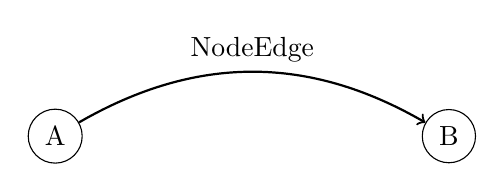
\begin{tikzpicture}
		\tikzset{vertex/.style = {shape=circle,draw,minimum size=.2em}}
		\tikzset{edge/.style = {->,> = latex'}}
		\node[vertex] (a) at  (0,0) {A};
		\node[vertex] (b) at  (5,0) {B};
		\path[->,draw,thick,bend left] (a) edge node[above] {NodeEdge} (b);
	\end{tikzpicture}
    \caption{Diagramm eines Sequenz-Knotens}
    \label{FIG:DiagramOneElementNode}
  \end{subfigure}
  \begin{subfigure}[c]{0.49\textwidth}
    \lstinputlisting[language=Java,caption={Java-Interface aus einem Sequenz-Knoten},label={LST:JInterfaceOneElementNode}]{Scope_one-element.java}
  \end{subfigure}
  \caption[Abbildung eines Sequenz-Knotens (\texttt{<rule> = NodeEdge;})]{Ein einzelner Sequenz-Knoten (\texttt{<rule> = NodeEdge;}) wird auf eine Methode in einem Interface abgebildet. Das Interface entspricht dem Scope am Anfang der gerichteten Kante.}
  \label{FIG:OneElementNode}
\end{figure}

\subsection{Sequenz von Knoten}\label{SEC:Sequence}
Tritt eine Sequenz von Knoten auf, muss für jeden Knoten ein Interface mit einer Methode generiert werden, um die Aufruf-Reihenfolge zu gewährleisten. Abbildung~\ref{FIG:SequenceNode} zeigt ein Beispiel mit zwei Knoten in einer Sequenz.
\begin{figure}[ht]
\centering
  \begin{subfigure}[c]{0.49\textwidth}
  	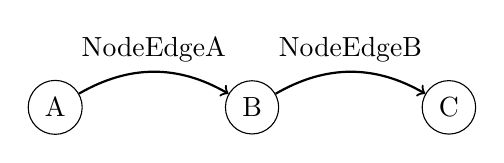
\begin{tikzpicture}
		\tikzset{vertex/.style = {shape=circle,draw,minimum size=.2em}}
		\tikzset{edge/.style = {->,> = latex'}}
		\node[vertex] (a) at  (0,0) {A};
		\node[vertex] (b) at  (2.5,0) {B};
		\node[vertex] (c) at  (5,0) {C};
		\path[->,draw,thick,bend left] (a) edge node[above] {NodeEdgeA} (b);
		\path[->,draw,thick,bend left] (b) edge node[above] {NodeEdgeB} (c);
	\end{tikzpicture}
    \caption{Diagramm einer Sequenz von Knoten}
    \label{FIG:DiagramSequenceNode}
  \end{subfigure}
  \begin{subfigure}[c]{0.49\textwidth}
    \lstinputlisting[language=Java,caption={Java-Interfaces aus einer Sequenz von Knoten},label={FIG:JInterfaceSequenceNode}]{Scope_sequence.java}
  \end{subfigure}
  \caption[Abbildung einer Sequenz (\texttt{<rule> = NodeEdgeA NodeEdgeB;})]{Eine Sequenz von Knoten (\texttt{<rule> = NodeEdgeA NodeEdgeB;}) wird auf eine Abfolge von Interfaces abgebildet, die jeweils eine Methode beinhalten, die das Folge-Interface als Rückgabewert haben.}
  \label{FIG:SequenceNode}
\end{figure}

\subsection{Kante mit Alternativen}\label{SEC:Alternative}
Alternativen in der EBNF können auf zwei Kanten von einem zu zwei verschiedenen Knoten abgebildet werden (siehe Abbildung~\ref{FIG:DiagramAlternativeNodeVariant}). Bei dieser Variante erhält jede Alternative einen eigenen End-Knoten. Das hat jedoch den Nachteil, dass wenn der Alternative in einer Sequenz weiter Elemente folgen, diese auf allen Pfaden der jeweiligen Alternativen dupliziert werden müssen.
\begin{figure}[ht]
\centering
  \begin{subfigure}[c]{0.49\textwidth}
  	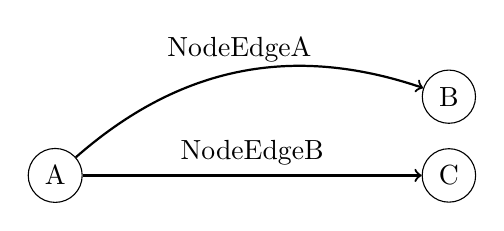
\begin{tikzpicture}
		\tikzset{vertex/.style = {shape=circle,draw,minimum size=.2em}}
		\tikzset{edge/.style = {->,> = latex'}}
		\node[vertex] (a) at  (0,0) {A};
		\node[vertex] (b) at  (5,1) {B};
		\node[vertex] (c) at  (5,0) {C};
		\path[->,draw,thick, bend left] (a) edge node[above] {NodeEdgeA} (b);
		\path[->,draw,thick] (a) edge node[above] {NodeEdgeB} (c);
	\end{tikzpicture}
    \caption{Diagramm alternativer Kanten}
    \label{FIG:DiagramAlternativeNodeVariant}
  \end{subfigure}
  \begin{subfigure}[c]{0.49\textwidth}
    \lstinputlisting[language=Java,caption={Java-Interface aus alternativen Kanten},label={LST:JInterfaceAlternativeNodeVariant}]{Scope_alternative_variant.java}
  \end{subfigure}
  \caption[Abbildung alternativer Kanten Variante 1]{Alternative Kanten (\texttt{<rule> = NodeEdgeA | NodeEdgeB;}) werden auf mehrere Methoden in einem Interface abgebildet, die verschiedene Rückgabetypen haben.}
  \label{FIG:AlternativeNodeVariant}
\end{figure}

Deshalb werden stattdessen die Alternativen auf parallele Kanten zwischen zwei Knoten abgebildet (siehe Abbildung~\ref{FIG:DiagramAlternativeNode}). Dadurch können die Alternativen jeweils wie Sequenzen zwischen dem selben Start- und End-Knoten abgebildet werden.
\begin{figure}[ht]
\centering
  \begin{subfigure}[c]{0.49\textwidth}
  	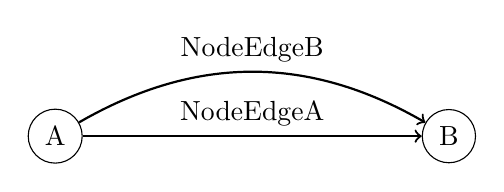
\begin{tikzpicture}
		\tikzset{vertex/.style = {shape=circle,draw,minimum size=.2em}}
		\tikzset{edge/.style = {->,> = latex'}}
		\node[vertex] (a) at  (0,0) {A};
		\node[vertex] (b) at  (5,0) {B};
		\path[->,draw,thick] (a) edge node[above] {NodeEdgeA} (b);
		\path[->,draw,thick, bend left] (a) edge node[above] {NodeEdgeB} (b);
	\end{tikzpicture}
    \caption{Diagramm alternativer Kanten}
    \label{FIG:DiagramAlternativeNode}
  \end{subfigure}
  \begin{subfigure}[c]{0.49\textwidth}
    \lstinputlisting[language=Java,caption={Java-Interface aus alternativen Kanten},label={LST:JInterfaceAlternativeNode}]{Scope_alternative.java}
  \end{subfigure}
  \caption[Abbildung alternativer Kanten Variante 2]{Alternative Kanten (\texttt{<rule> = NodeEdgeA | NodeEdgeB;}) werden auf mehrere Methoden in einem Interface abgebildet, die denselben Rückgabewert haben.}
  \label{FIG:AlternativeNode}
\end{figure}

\subsection{Optionales Element}\label{SEC:Optional}
Im Falle eines optionalen Elementes, muss auch der Methodenaufruf optional sein und auch der nächstfolgende Methodenaufruf verfügbar sein. Das wird dadurch erreicht, indem das erste Interface vom folgenden erbt. Im Graphen wird das durch eine parallele Kante eines anderen Typen (OptionalEdge in Abbildung~\ref{FIG:DiagramOptionalNode}) repräsentiert. Listing~\ref{LST:JInterfaceOptionalNode}) ist, bis auf die Vererbung, gleich zu Listing~\ref{LST:JInterfaceOneElementNode}.
\begin{figure}[ht]
\centering
  \begin{subfigure}[c]{0.49\textwidth}
  	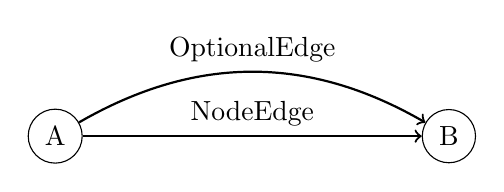
\begin{tikzpicture}
		\tikzset{vertex/.style = {shape=circle,draw,minimum size=.2em}}
		\tikzset{edge/.style = {->,> = latex'}}
		\node[vertex] (a) at  (0,0) {A};
		\node[vertex] (b) at  (5,0) {B};
		\path[->,draw,thick] (a) edge node[above] {NodeEdge} (b);
		\path[->,draw,thick, bend left] (a) edge node[above] {OptionalEdge} (b);
	\end{tikzpicture}
    \caption{Diagramm einer optionalen Kante}
    \label{FIG:DiagramOptionalNode}
  \end{subfigure}
  \begin{subfigure}[c]{0.49\textwidth}
    \lstinputlisting[language=Java,caption={Java-Interface aus einer optionalen Kante},label={LST:JInterfaceOptionalNode}]{Scope_optional.java}
  \end{subfigure}
  \caption[Abbildung eines optionalen Elements (\texttt{<rule> = [NodeEdgeA];})]{Ein optionales Element (\texttt{<rule> = [NodeEdgeA];}) wird auf ein Interface mit einer Methode, die das Folge-Interface zurück gibt, abgebildet. Das Interface erbt auch vom Folge-Interface um den Methodenaufruf zu überspringen.}
  \label{FIG:OptionalNode}
\end{figure}

\subsection{Kante mit optionaler Schleife}\label{SEC:OptionalLoop}
Da die Wiederholung bei EBNF optional ist (beliebig oft oder keinmal auftreten darf), gibt es hier, wie beim optionalen Element eine Kante vom Typ OptionalEdge. Dadurch kann der Methodenaufruf übersprungen werden.

Um den Methodenaufruf wiederholbar zu machen kann man nicht einfach eine parallele, optionale Kante in die entgegengesetzte Richtung einfügen, weil diese ebenfalls in eine Vererbung umgesetzt würde; dadurch würde zwischen beiden Interfaces eine zirkuläre Abhängigkeit entstehen, die in Java verboten ist.

Stattdessen wird bei der optionalen Wiederholung die Kante, die den Methodenaufruf repräsentiert, eine Schleife zum Knoten selbst. Somit kann die Methode beliebig oft aufgerufen werden, bevor die in B deklarierte Methode aufgerufen wird (Abbildung~\ref{FIG:DiagramLoopNode}).
\begin{figure}[ht]
\centering
  \begin{subfigure}[c]{0.49\textwidth}
  	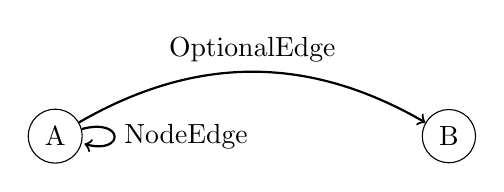
\begin{tikzpicture}
		\tikzset{vertex/.style = {shape=circle,draw,minimum size=.2em}}
		\tikzset{edge/.style = {->,> = latex'}}
		\node[vertex] (a) at  (0,0) {A};
		\node[vertex] (b) at  (5,0) {B};
		\path[->,draw,thick, bend left] (a) edge node[above] {OptionalEdge} (b);
		\path[->,draw,thick, loop right] (a) edge node[right] {NodeEdge} (a);
	\end{tikzpicture}
    \caption{Diagramm einer Schleifen-Kante (Variante 1)}
    \label{FIG:DiagramLoopNode}
  \end{subfigure}
  \begin{subfigure}[c]{0.49\textwidth}
    \lstinputlisting[language=Java,caption={Java-Interface aus einer Schleifen-Kante (Variante 1)},label={LST:JInterfaceLoopNode}]{Scope_loop.java}
  \end{subfigure}
  \caption[Abbildung einer optionalen Schleife (Variante 1)]{Eine optionale Schleifen (\texttt{<rule> = \{NodeEdge\};}) kann auf ein Interface mit einer Methode mit dem Interface selbst als Rückgabewert und vom Folge-Interface erbend abgebildet werden. (Variante 1)}
  \label{FIG:LoopNode}
\end{figure}

Eine zweite Variante benötigt einen Hilfsknoten (Knoten B in Abbildung~\ref{FIG:DiagramLoopNodeAlt}). Im trivialen Fall ist dieser Hilfskonten unnötig, befindet sich die Schleife innerhalb einer Alternative sichert er aber die Wiederholung der richtigen Kante(n) (siehe Abbildung~\ref{FIG:LoopInAlternative}).
\begin{figure}[ht]
\centering
  \begin{subfigure}[c]{0.49\textwidth}
  	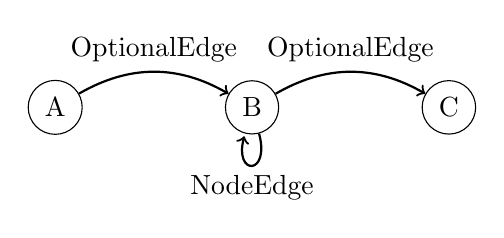
\begin{tikzpicture}
		\tikzset{vertex/.style = {shape=circle,draw,minimum size=.2em}}
		\tikzset{edge/.style = {->,> = latex'}}
		\node[vertex] (a) at  (0,0) {A};
		\node[vertex] (b) at  (2.5,0) {B};
		\node[vertex] (c) at  (5,0) {C};
		\path[->,draw,thick, bend left] (a) edge node[above] {OptionalEdge} (b);
		\path[->,draw,thick, loop below] (b) edge node[below] {NodeEdge} (b);
		\path[->,draw,thick, bend left] (b) edge node[above] {OptionalEdge} (c);
	\end{tikzpicture}
    \caption{Diagramm einer Schleifen-Kante (Variante 2)}
    \label{FIG:DiagramLoopNodeAlt}
  \end{subfigure}
  \begin{subfigure}[c]{0.49\textwidth}
    \lstinputlisting[language=Java,caption={Java-Interface aus einer Schleifen-Kante (Variante 2)},label={LST:JInterfaceLoopNodeAlt}]{Scope_loop_alt.java}
  \end{subfigure}
  \caption[Abbildung einer optionalen Schleife (Variante 2)]{Eine optionale Schleifen (\texttt{<rule> = \{NodeEdge\};}) kann auf zwei Interfaces abgebildet werden. Das erste ist ein Hilf-Interface, das vom eigentlichen erbt, das zweite enthält die Methode, die das Interface selbst als Rückgabewert zurück gibt. (Variante 2)}
  \label{FIG:LoopNodeAlt}
\end{figure}


\subsection{Schachtelung der Konstrukte}
In diesem Abschnitt wird darauf eingegangen, wie die Rekursion der ENBF-Konstrukte behandelt werden können. Die Fälle von Alternative und Schleifen in einer Sequenz werden aus Trivialität übersprungen. Hier soll nur auf Fälle eingegangen werden, die nicht aus den vorherigen Beispielen ersichtlich sind.

\subsubsection{Sequenz in einer Schleife}
Befindet sich eine Sequenz in einer Schleife, bilden die Knoten und Kanten eine Schleife zum Ziel-Knoten (Abbildung~\ref{FIG:DiagramSequenceInLoop}) der Schleife analog zur trivialen Variante der Schleife (siehe Abbildung~\ref{FIG:DiagramLoopNode}).
\begin{figure}[ht]
\centering
  \begin{subfigure}[c]{0.49\textwidth}
  	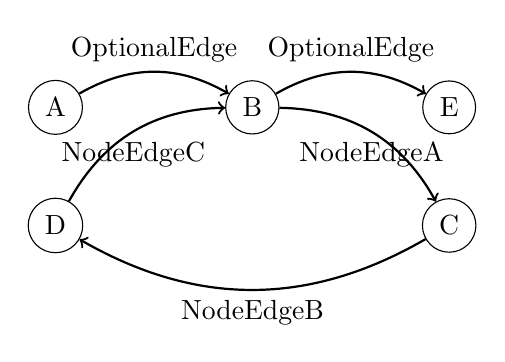
\begin{tikzpicture}
		\tikzset{vertex/.style = {shape=circle,draw,minimum size=.2em}}
		\tikzset{edge/.style = {->,> = latex'}}
		\node[vertex] (a) at  (0,0) {A};
		\node[vertex] (b) at  (2.5,0) {B};
		\node[vertex] (c) at  (5,-1.5) {C};
		\node[vertex] (d) at  (0,-1.5) {D};
		\node[vertex] (e) at  (5,0) {E};
		\path[->,draw,thick, bend left] (a) edge node[above] {OptionalEdge} (b);
		\path[->,draw,thick, bend left] (b) edge node[above] {OptionalEdge} (e);
		\path[->,draw,thick, bend left] (b) edge node[below] {NodeEdgeA} (c);
		\path[->,draw,thick, bend left] (c) edge node[below] {NodeEdgeB} (d);
		\path[->,draw,thick, bend left] (d) edge node[below] {NodeEdgeC} (b);
	\end{tikzpicture}
    \caption{Diagramm einer Sequenz innerhalb eines Schleifen-Knotens}
    \label{FIG:DiagramSequenceInLoop}
  \end{subfigure}
  \begin{subfigure}[c]{0.49\textwidth}
    \lstinputlisting[language=Java,caption={Java-Interface aus einer Sequenz in einem Schleifen-Knoten},label={LST:JInterfaceSequenceInLoop}]{Sequence_in_loop.java}
  \end{subfigure}
  \caption[Abbildung einer Sequenz innerhalb einer Schleife]{Eine Sequenz innerhalb einer Schleife (\texttt{<rule> = \{NodeEdgeA NodeEdgeB NodeEdgeC\};}) ersetzt dessen einfache Kante zum Knoten selbst. Für jeden Scope in der Sequenz muss ein eigenes Interface erstellt werden. (nach Variante 2)}
  \label{FIG:SequenceInLoop}
\end{figure}

\subsubsection{Alternative in einer Schleife}
Befindet sich eine Alternative in einer Schleife, werden alle Alternativen, die nur aus einer Kante bestehen, in eine Schleifen-Kante am Ziel-Knoten der Schleife transformiert. Besteht eine Alternative aus einer Sequenz, wird aus dieser Sequenz eine weitere Schleife aus mehreren Kanten und Knoten (siehe Abbildung~\ref{FIG:DiagramAlternativeInLoop}).

Falls die Alternative sich in einer Sequenz in einer Alternative befindet, gibt es in der Schleife mehrere ausgehende Kanten vom Ziel-Knoten der Schleife.
\begin{figure}[ht]
\centering
  \begin{subfigure}[c]{0.49\textwidth}
  	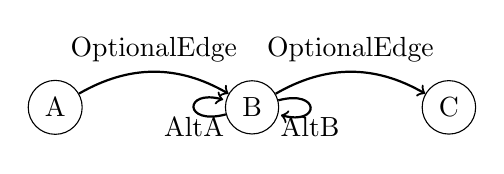
\begin{tikzpicture}
		\tikzset{vertex/.style = {shape=circle,draw,minimum size=.2em}}
		\tikzset{edge/.style = {->,> = latex'}}
		\node[vertex] (a) at  (0,0) {A};
		\node[vertex] (b) at  (2.5,0) {B};
		\node[vertex] (c) at  (5,0) {C};
		\path[->,draw,thick, bend left] (a) edge node[above] {OptionalEdge} (b);
		\path[->,draw,thick, bend left] (b) edge node[above] {OptionalEdge} (c);
		\path[->,draw,thick, loop left] (b) edge node[below] {AltA} (b);
		\path[->,draw,thick, loop right] (b) edge node[below] {AltB} (b);
	\end{tikzpicture}
    \caption{Diagramm einer Alternative innerhalb eines Schleifen-Knotens}
    \label{FIG:DiagramAlternativeInLoop}
  \end{subfigure}
  \begin{subfigure}[c]{0.49\textwidth}
    \lstinputlisting[language=Java,caption={Java-Interfaces aus einer Alternative in einer Schleife},label={LST:JInterfaceAlternativeInLoop}]{Loop_with_inner_alternative.java}
  \end{subfigure}
  \caption[Abbildung einer Alternative innerhalb einer Schleife]{Diagramm und Interface einer Alternative innerhalb eines Schleifen-Knotens (nach Variante 2) (\texttt{<rule> = \{(AlternativeA | AlternativeB)\};})}
  \label{FIG:AlternativeInLoop}
\end{figure}

\subsubsection{Schleife in Alternative}
Befindet sich eine Schleife in einer Alternative, muss für ihre Kante ein Hilfsknoten eingeführt werden, auch wenn die Schleife nur eine Kante beinhaltet (Knoten C in Abbildung~\ref{FIG:DiagramLoopInAlternative}). Würde man die optionalen Kante direkt von A nach B aufnehmen, wären NodeEdgeB und NodeEdgeC ebenfalls optional und würde nicht dem EBNF-Konstrukt entsprechen.
\begin{figure}[ht]
\centering
  \begin{subfigure}[c]{0.49\textwidth}
  	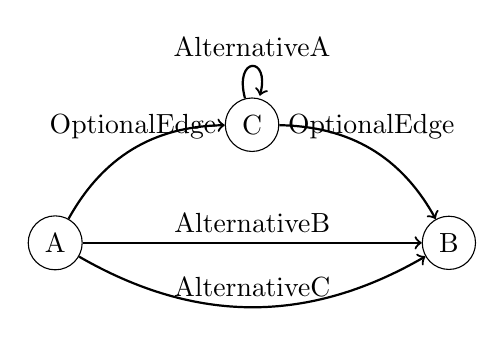
\begin{tikzpicture}
		\tikzset{vertex/.style = {shape=circle,draw,minimum size=.2em}}
		\tikzset{edge/.style = {->,> = latex'}}
		\node[vertex] (a) at  (0,0) {A};
		\node[vertex] (b) at  (5,0) {B};
		\node[vertex] (c) at  (2.5,1.5) {C};
		\path[->,draw,thick, bend left] (a) edge node[above] {OptionalEdge} (c);
		\path[->,draw,thick, loop above] (c) edge node[above] {AlternativeA} (c);
		\path[->,draw,thick, bend left] (c) edge node[above] {OptionalEdge} (b);
		\path[->,draw,thick] (a) edge node[above] {AlternativeB} (b);
		\path[->,draw,thick, bend right] (a) edge node[above] {AlternativeC} (b);
	\end{tikzpicture}
    \caption{Diagramm einer Schleife innerhalb einer Alternative}
    \label{FIG:DiagramLoopInAlternative}
  \end{subfigure}
  \begin{subfigure}[c]{0.49\textwidth}
    \lstinputlisting[language=Java,caption={Java-Interface aus einer Schleife innerhalb einer Alternative},label={LST:JInterfaceLoopInAlternative}]{Alternative_with_inner_loop.java}
  \end{subfigure}
  \caption[Abbildung einer Schleife innerhalb einer Alternative]{Diagramm und Interface einer Schleife innerhalb einer Alternative (\texttt{<rule> = \{NodeEdgeA\} | NodeEdgeB | NodeEdgeC;})}
  \label{FIG:LoopInAlternative}
\end{figure}

\subsubsection{Schleifen in Alternative}
Befinden sich mehrere Schleifen innerhalb einer Alternative, werden mehrere ausgehende optionale Kanten zu einem Knoten angelegt (siehe Abbildung~\ref{FIG:DiagramLoopsInAlternative}). Daher kann statt Interfaces keine abstrakten Klassen verwendet werden; in Scala, das keine Interfaces kennt, müssen daher Traits statt abstrakten Klassen verwendet werden.
\begin{figure}[ht]
\centering
  \begin{subfigure}[c]{0.49\textwidth}
  	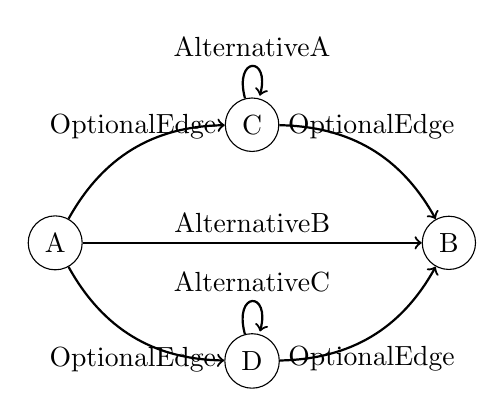
\begin{tikzpicture}
		\tikzset{vertex/.style = {shape=circle,draw,minimum size=.2em}}
		\tikzset{edge/.style = {->,> = latex'}}
		\node[vertex] (a) at  (0,0) {A};
		\node[vertex] (b) at  (5,0) {B};
		\node[vertex] (c) at  (2.5,1.5) {C};
		\node[vertex] (d) at  (2.5,-1.5) {D};
		\path[->,draw,thick, bend left] (a) edge node[above] {OptionalEdge} (c);
		\path[->,draw,thick, loop above] (c) edge node[above] {AlternativeA} (c);
		\path[->,draw,thick, bend left] (c) edge node[above] {OptionalEdge} (b);
		\path[->,draw,thick] (a) edge node[above] {AlternativeB} (b);
		\path[->,draw,thick, bend right] (a) edge node[below] {OptionalEdge} (d);
		\path[->,draw,thick, loop above] (d) edge node[above] {AlternativeC} (d);
		\path[->,draw,thick, bend right] (d) edge node[below] {OptionalEdge} (b);
	\end{tikzpicture}
    \caption{Diagramm einer Schleife innerhalb einer Alternative}
    \label{FIG:DiagramLoopsInAlternative}
  \end{subfigure}
  \begin{subfigure}[c]{0.49\textwidth}
    \lstinputlisting[language=Java,caption={[Java-Interface aus zwei Schleifen innerhalb einer Alternative]Java-Interface aus zwei Schleifen innerhalb einer Alternative. Da hier mehrere ausgehende optionale Kanten bei einem Knoten auftreten wird von mehreren Interfaces geerbt.},label={LST:JInterfaceLoopsInAlternative}]{Alternative_with_inner_loops.java}
  \end{subfigure}
  \caption[Abbildung mehrere Schleifen innerhalb einer Alternative]{Diagramm und Interface einer Schleife innerhalb einer Alternative (\texttt{<rule> = \{NodeEdgeA\} | NodeEdgeB | \{NodeEdgeC\};})}
  \label{FIG:LoopsInAlternative}
\end{figure}

\subsection{Scala}
Da es in Scala keine Interfaces gibt, kommen entweder abstrakte Klassen oder Traits infrage. Da mehrere Schleifen in einer Alternative Mehrfachvererbung voraussetzen (siehe Abbildung~\ref{FIG:LoopsInAlternative}), scheiden die abstrakten Klassen aus.

Es werden also Traits generiert, die die selben Methoden wie die Interface-Pendants haben und (bis auf void, das auf Unit abgebildet wird) die gleichen Parameter- und Rückgabetypen haben, da die Java-Typen verwendet werden können.

Beispielhaft wird hier noch einmal die optionale Schleife aufgeführt (Abbildung~\ref{FIG:ScalaLoopNodeAlt}), um den generierten Scala-Code zu zeigen, weil bei der Schleife Methoden und Vererbung vorkommen.
\begin{figure}[ht]
\centering
  \begin{subfigure}[c]{0.49\textwidth}
  	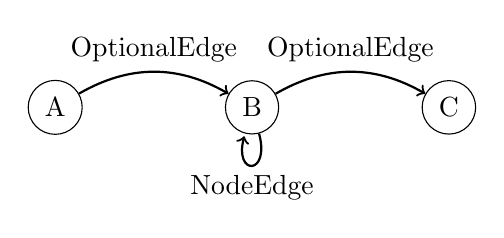
\begin{tikzpicture}
		\tikzset{vertex/.style = {shape=circle,draw,minimum size=.2em}}
		\tikzset{edge/.style = {->,> = latex'}}
		\node[vertex] (a) at  (0,0) {A};
		\node[vertex] (b) at  (2.5,0) {B};
		\node[vertex] (c) at  (5,0) {C};
		\path[->,draw,thick, bend left] (a) edge node[above] {OptionalEdge} (b);
		\path[->,draw,thick, loop below] (b) edge node[below] {NodeEdge} (b);
		\path[->,draw,thick, bend left] (b) edge node[above] {OptionalEdge} (c);
	\end{tikzpicture}
    \caption{Diagramm einer Schleifen-Kante (Variante 2)}
    \label{FIG:ScalaDiagramLoopNodeAlt}
  \end{subfigure}
  \begin{subfigure}[c]{0.49\textwidth}
    \lstinputlisting[language=Scala,caption={Scala-Trait aus einer Schleifen-Kante (Variante 2)},label={LST:ScalaTraitLoopNodeAlt}]{Scope_loop_alt.scala}
  \end{subfigure}
  \caption[Abbildung einer Sequenz auf einen Sala-Trait]{Diagramm und Interface einer Schleifen-Kante (Variante 2) (\texttt{<rule> = \{NodeEdge\};})}
  \label{FIG:ScalaLoopNodeAlt}
\end{figure}


\section{Generierung der Interfaces}
Die Java-Interfaces und Scala-Traits werden mit StringTemplate generiert, die aus dem ANTLR-Projekt hervorging~\cite{stringtemplate.github} und die von Parr auch vorgeschlagen werden~\cite[S. 313 ff]{Parr.2010}. Zwar gibt es auch andere Template-Engines (z.B. Apache Velocity\footnote{\url{http://velocity.apache.org/}}), aber StringTemplate biete eine bessere Trennung von Daten und Template~\cite{parr2004enforcing}.

Listing~\ref{LST:STJavaInterface} zeigt das Template für Java-Interfaces das ein Interface mit beliebig vielen Super-Interfaces und Methoden erzeugen kann. Das Template für Scala-Traits ist analog aufgebaut, mit dem Unterschied, dass die Reihenfolge der Argumentnamen und -typen unterschiedlich ist und das Interface durch Trait ersetzt wurde.

Um das Template zu instantiieren muss die Template-Datei geladen und eine Instanz eines Templates (per Namen) erstellt werden (Listing~\ref{LST:STInstantiation}, Zeilen 2 und 3); danach können die Argumente des Templates gesetzt werden (Listing~\ref{LST:STJavaInterface} Zeile 1, Listing~\ref{LST:STInstantiation} Zeilen 4-7). Da StringTemplate die Argument per Lazy Evaluation anwendet wird der Text erst beim Aufruf der Render-Methode ersetzt (Listing~\ref{LST:STInstantiation} Zeile 8) und somit Kollisionen mit dem Inhalt der Argumente vermieden.
\begin{lstlisting}[language=,caption={String-Template für ein Java-Interface mit Methoden},label=LST:STJavaInterface]
javaInterface(package,interfaceName,parents,methods) ::= <<
package <package>;

public interface <interfaceName> <if(parents)>extends <parents;separator=", "> <endif> {<methods:{method|<javaMethod(method.returnType,method.name,method.arguments)>}>
}

>>

javaMethod(returnType,name,arguments) ::= <<

    <returnType> <name>(<arguments:{argument|<argument.type> <argument.name>};separator=", ">);
>>
\end{lstlisting}

\begin{lstlisting}[caption={Instantiierung eines String-Templates},label=LST:STInstantiation]
String renderInterface(final Interface anInterface) {
    final STGroup stGroup = new STGroupFile("java_interface.stg");
    return stGroup.getInstanceOf(javaInterface)
        .add("package", getTargetPackage())
        .add("interfaceName", anInterface.getName())
        .add("methods", anInterface.getMethods())
        .add("parents", anInterface.getParents())
        .render();
}
\end{lstlisting}

\subsection{Kollisionen mit Elementen der Hostsprache}
Durch die in der EBNF gewählten Bezeichner können Kollisionen mit den Schlüsselworten und Typen auftreten. Darauf sollte schon beim Schreiben der EBNF geachtet werden, falls die Zielsprache bekannt ist. Trotzdem werden schon beim Erstellen der Interfaces Kollisionen vermieden, indem die Bezeichner und generierten Interfacenamen überprüft werden.

Vor dem Speichern der Interfaces wird geprüft, ob die Interface-, Methoden- und Argumentnamen Schlüsselworte oder Typen von Java und Scala sind. Bei Kollisionen von Interfacenamen wird der interne Bezeichner angehängt, bei Methodennamen kann \gqq{Method} angehängt werden, und bei Argumentnamen wird ein \gqq{an} vorangestellt und der eigentliche Name im Camelcase angehängt. Die Argument-Typen dürfen auch Typen der Hostsprache sein, aber kein Schlüsselwort.

\subsection{Benennung der Interfaces}
Die Scopes erhalten im Graphen interne, eindeutige Bezeichner; diese könnten als Namen für die Interfaces verwendet werden, da bis auf das Start-Interfaces alle nicht instantiiert werden, sondern nur deren Methoden aufgerufen oder implementiert werden. Da der Start- und End-Scope des Graphen eindeutig bestimmbar sind, werden diese mit BeginScope respekive EndScope benannt.

Um die restlichen Interfaces trotzdem mit sprechenden Namen zu versehen, werden die Namen der Methoden und \gqq{Scope} aneinander gehängt, wobei die Namenskonvention von Java (Camelcase) eingehalten wird. Dabei gibt es, bis auf eine Ausnahme, für jedes Interface mindestens eine Methode, die zur Namensgenerierung verwendet werden kann (siehe Abschnitte~\ref{SEC:OneNode}~bis~\ref{SEC:OptionalLoop}). Nur die Scopes, die direkt vor einer optionalen Wiederholung auftreten, haben keine ausgehende Kante vom Typ NodeEdge (seihe Abschnitt~\ref{SEC:OptionalLoop}); für diese Interfaces muss der interne Bezeichner aus dem Graphen als Interfacename gewählt werden.

Auch können Kollisionen vorkommen, etwa wenn ein Nicht-Terminal oder ein Keyword mehrfach vorkommt. Dann wäre der Name für das Interface nicht mehr eindeutig und es wird der interne Bezeichner des Scopes aus dem Graphen an das beschriebene Schema angehängt. Somit bleibt der Name des Interfaces eindeutig, da die Bezeichner innerhalb des Graphen eindeutig gewählt wurden.

Da die Methodennamen aneinander gehängt werden, können für die Interfaces Namen vorkommen, die länger als üblich sind. Für Java selbst stellt das kein Problem dar (siehe~\cite[S. 24]{javalanguagespecification.oracle}), für den Benutzer der DSL könnte das aber suboptimal sein; jedoch ist ein lesbarer Name besser als ein interner Bezeichner des Graphen.

\subsection{Benennung der Methoden}
Die Namen der Methoden werden direkt aus der Kante vom Typ \gqq{Keyword} generiert. Es wird überprüft, ob der Name ein Schlüsselwort oder Typ der Hostsprache ist, und in dem Fall eine Suffix angehängt.

\subsection{Benennung der Argumente}
Die Argumente werden aus der Kante vom Typ \gqq{Type} generiert, die der Kante einer Methode folgt. Der Typ des Arguments entspricht dem Bezeichner aus der EBNF, der Name wird aus dem Typ abgeleitet: der erste Buchstabe wird zum Kleinbuchstaben, und falls dieser Name ebenfalls ein Typ oder Schlüsselwort ist, wird ein \gqq{an} vorangestellt.

\section{Schwierigkeiten beim Bau}
Beim Erstellen des Prototypen traten einige Schwierigkeiten auf. Die größten werden in diesem Abschnitt besprochen: die Behandlung der Rekursion der EBNF-Grammatik und die der Typen.

\subsection{Einschränkungen der Grammatik}
Die EBNF-Grammatik kann nicht beliebig formuliert sein, es gibt folgende Einschränkungen:
\begin{itemize}
	\item Für alle Nicht-Terminale muss es eine Regel mit demselben Namen geben
	\item Eine Kante vom Typ \gqq{Type} muss einer vom Typ \gqq{Keyword} vorangehen,
	\item Eine Methoden kann höchstens ein Argument haben
	\item Eine Start-Regel muss definiert werden
	\item Lexer-Regeln für die Umsetzung der Tokens
	\item Methodennamen können nicht beliebig gewählt werden
\end{itemize}

\subsection{Nicht-Terminale}
Alle Nicht-Terminale, die in der Grammatik vorkommen, müssen in derselben Grammatik eine entsprechende Regel haben. Diese Regel muss den gleichen Namen wie das zu ersetzende Nicht-Terminal haben, damit es durch die Regel ersetzt werden kann. Da in dem Prototypen nicht mehrere Grammatiken verarbeitet werden können, muss die Regel in der gleichen Grammatik stehen.

Ansonsten muss sich die zu ersetzende Regel an die restlichen (folgenden) Einschränkungen halten. Auch muss beachtet werden, dass nach dem Ersetzen einer Regel nicht zwei Kanten vom Typ \gqq{TYPE} nicht aufeinander folgen.

\subsubsection{Folge von Type auf Keyword}\label{SEC:TypeFollowsKeyword}
Um die Schlüsselworte der Sprache umzusetzen, werden die Keywords aus der EBNF auf Methoden abgebildet, und die Typen aus der EBNF auf Typen der Hostsprache (oder eigens definierte Typen). Deshalb ergibt es innerhalb der in diesem Kontext geschriebener EBNF keinen Sinn, wenn ein Keyword nicht einem Typ vorangeht.

\subsubsection{Methode mit einem Argument}
Mit Abschnitt~\ref{SEC:TypeFollowsKeyword} hängt das Auftreten und die Anzahl der Argumente zusammen. Die einfachste Möglichkeit ist es nur ein Argument zuzulassen, indem einem Keyword nur ein Typ folgen darf, der das Argument darstellt. Es ist auch möglich eine Folge von Typen an ein Keyword anzuhängen, das wird vom Prototypen aber noch nicht unterstützt.

\subsubsection{Startregel}
In der Grammatik muss eine Startregel definiert sein, die auf der rechten Seite nur ein Nicht-Terminal beinhaltet. Diese Regel wird als Einstiegspunkt für das Ersetzen der Graphen der Nicht-Terminalen verwendet.

\subsubsection{Lexer-Regeln}
Für jede Lexer-Regel sollte es eine entsprechende Parser-Regel geben, die nur die jeweilige Lexer-Regel beinhaltet. Dadurch kann der Listener des Parsers die Typen auch verarbeiten.

Falls eine Regel innerhalb einer anderen vorkommt, ohne ein Trennsymbol zu einer anderen, darf es ebenfalls keine Lexer-Regel sein, um vom Listener erkannt zu werden.

\subsubsection{Methodennamen}
Die Schlüsselwörter in der EBNF, die auf Methodennamen abgebildet werden, können nicht beliebig gewählt werden, da Kollisionen mit der Hostsprache auftreten dürfen. Schlüsselworte und (benutzerdefinierte) Typen dürfen nicht verwendet werden. Schlüsselworte von Java uns Scala und die primitiven Datentypen werden erkannt und erzeugen eine Fehlermeldung. Benutzerdefinierte Typen müssen schon beim Schreiben der Grammatik selbst vermieden werden.


\subsection{Behandlung der Rekursion}
Die in der EBNF-Grammatik vorkommende Rekursion (Alternative in Wiederholung in Sequenz in Alternative) wird korrekt behandelt, um den korrekten Parse-Tree zu erstellen. Auch können die Nicht-Terminale durch ihre Repräsentation aus derselben Grammatik richtig ersetzt werden.

Jedoch können Grammatiken nicht ineinander geschachtelt werden; das könnte dazu verwendet werden um durch eine Grammatik einen Typen zu generieren, der in einer anderen als Typ eines Arguments vorkommt.

Stattdessen kann man mit dem Prototypen eine Grammatik verarbeiten, dessen letztes Interface mit der End-Methode ein Objekt vom einem spezifiziertem Typ zurück liefert (siehe Parameter~\gqq{-r}\footnote{\url{https://github.com/etgramli/AntlrTest}}). Diesen Rückgabetyp kann man als Typ für ein Argument in einer anderen Grammatik verwenden.

\subsection{Nicht-Terminale}
Nicht-Terminale werden durch ihre Entsprechung aus Terminalen ersetzt, danach werden die Terminale durch die folgenden Regeln abgebildet.

\subsection{Scope-Namen}
Die Sopes werden zunächst durch den Graphen selbst erstellt und nummeriert. Diese Namen könnte man beibehalten, da die Bezeichner der Interfaces nicht direkt benutzt werden (bis auf das Start- und End-Interface).

Um trotzdem sprechende Namen zu vergeben, können die Namen der Methoden des Interfaces bestimmt und diese aneinander gehängt werden. Da das zu Kollisionen führen kann, wird in dem Fall der (eindeutige) Name des Scopes aus dem Graphen am Schluss angehängt.


\chapter{Testlauf mit anschaulichem Beispiel}\label{SEC:Example}
In diesem Kapitel wird die Benutzung des Prototypen\footnote{\url{https://github.com/etgramli/AntlrTest}} anhand von zwei Beispielen dokumentiert. Zuerst werden Interfaces für mathematische Ausdrücke generiert, und dann ein Beispiel eines Typsystems vorgestellt.

\section{Verwendung des Prototypen}
Der Prototyp kann entweder als eigenständige Anwendung in der Kommandozeile verwendet oder als Maven-Abhängigkeit eingebunden werden\footnote{\url{https://github.com/etgramli/AntlrTest/packages/145801}}. Die Abhängigkeit kann zum Beispiel verwendet werden um die Klasse, die die Interfaces bzw. Traits als Dateien schreibt, für eine neue Hostsprache zu erweitern. In diesem Kapitel wird nur die Benutzung des Prototypen beschrieben; die Kommandozeilenargumente sind in Tabelle~\ref{TAB:PrototypeCMD} aufgeführt (und werden auf der Projektseite\footnote{\url{https://github.com/etgramli/AntlrTest}} genauer beschrieben). Für die hier vorgestellten Beispiele sind nur die ersten vier Parameter wichtig. Zusätzlich werden die mit der Option -s generierten Graphen angegeben, für die Funktionalität des Prototyps selbst ist sie aber nicht wichtig.

\begin{table}[ht]
\centering
\begin{tabular}{llll}
\multicolumn{2}{c|}{\textbf{Option}} & & \\
\textbf{Kurz} & \multicolumn{1}{c|}{\textbf{Lang}} & \textbf{Argument} & \textbf{Pflicht}\\\hline
-d & --directory    & Pfad zu Ordner  & Ja\\
-p & --package      & Java-Package    & Ja\\
-g & --grammar      & Grammatik-Datei & Ja\\
-r & --return-type  & String          & Nein\\
-j & --java         & <keins>         & Nein\\
-c & --scala        & <keins>         & Nein\\
-s & --sketch-graph & Dateiname       & Nein\\
-h & --help         & <keins>         & Nein\\
\end{tabular}
\caption{Kommandozeilenargumente des Prototypen}
\label{TAB:PrototypeCMD}
\end{table}

\section{Mathematische Ausdrücke}
Das erste Beispiel, an dem der Prototyp demonstriert wird, soll ein gängiges sein. Deswegen wurde dafür mathematische Ausdrücke ausgewählt. Listing~\ref{LST:EXPRBNF} zeigt die Definition der Ausdrücke als EBNF. Hier wird für jede Grundrechenart eine Regel deklariert, die die je eine Alternative mit dem Typ Double und Expr enthält, der als Rückgabetyp des Programms angegeben werden kann.

Mit dem Prototypen\footnote{\url{https://github.com/etgramli/AntlrTest}} kann mit einem Aufruf auch ein Graphen wie in Abbildung~\ref{FIG:ExprGraph} generiert werden. Der Aufruf kann zum Beispiel so aussehen:
\begin{lstlisting}
java -jar antlr-test-1.6.1-jar-with-dependencies.jar -d targetDir -p com.package.expr -g expr.bnf -s exprGraph.dot -r Expr
\end{lstlisting}

\begin{figure}
\lstinputlisting[language=Java,caption={Expression-EBNF (expr.bnf)},label={LST:EXPRBNF}]{expr.bnf}
\end{figure}

Der generierte DOT-Graph kann mit z.B. einem Online-Tool\footnote{\url{https://dreampuf.github.io/GraphvizOnline/}} visualisiert werden, um einen Überblick über die Aufruf-Reihenfolge zu erhalten. Der Graph in Abbildung~\ref{FIG:ExprGraph} zeigt den aus der EBNF-Grammatik generierten Graphen. Wie zuvor beschrieben wurden hierfür alle Nicht-Terminale durch ihre entsprechenden Regeln ersetzt wodurch nur ein zusammenhängender Graph entsteht; die Regel \verb|<expr>| diente hierbei als Einstiegs-Regel.

\begin{figure}[ht]
\centering
\resizebox{\linewidth}{!}{\input{\main/10_Pictures/expr.tex}}
\caption{Graph generiert aus der Expression-EBNF}
\label{FIG:ExprGraph}
\end{figure}

In diesem Graphen werden noch keine sprechenden Namen verwendet, sondern es werden die graph-internen Bezeichnungen der Scopes verwendet. Die aussagekräftigen Namen werden erst beim Generieren der Interfaces generiert, da erst hier auf Kollisionen mit Typen und Schlüsselworten der Hostsprache überprüft wird. Tabelle~\ref{TAB:MappingExpressionScopeToInterface} zeigt welche Namen der Interfaces im Vergleich mit den Namen der zugehörigen Scopes.

Man sieht hier auch, dass nicht zu jedem Knoten des Graphen ein eigenes Interfaces generiert wird. Da die Kanten vom Typ \gqq{KEYWORD} auf Methoden abgebildet werden, werden folgende TYP-Kanten auf Argumente abgebildet; der Knoten dazwischen repräsentiert also kein Interface und erhält auch keinen sprechenden Namen. Knoten, die nur ausgehende, optionale Kanten haben (z.B. Scope3 in Abbildung~\ref{FIG:ExprGraph}), erhalten ebenfalls keinen sprechenden Namen, da es für diese Knoten keine Methoden gibt, aus denen der Name generiert wird. Der End-Scope ohne ausgehende Kanten würde nach der Regel ebenfalls keinen Namen erhalten, wird aber stets \gqq{EndScope} genannt, da es nur einen solchen Scope gibt (siehe~\ref{SEC:Alternative}).

\begin{table}[ht]
\centering
\begin{tabular}{ll}
\textbf{Name des Scopes} & \textbf{Name des Interfaces}\\\hline
Scope0 & BeginScope\\
Scope3 & Scope3\\
Scope5 & DividedMinusPlusTimesScope\\
Scope1 & EndScope\\
\end{tabular}
\caption[Abbildung von Scope- auf Interfacenamen (Expression-Beispiel)]{Abbildung von Scope- auf Interface-Namen (Expression-Beispiel)}
\label{TAB:MappingExpressionScopeToInterface}
\end{table}

\subsection{Generierte Interfaces}
Die folgenden Interfaces werden für den in Abbildung~\ref{FIG:ExprGraph} gezeigten Graphen generiert. Die Namen der Interfaces entsprechen jetzt, bis auf Scope3, nicht mehr den Bezeichnern der Scopes im Graphen. Die Methodennamen wurden den Namen der Kanten vom Typ \gqq{KEYWORD} entnommen. Die Namen der Argumente wurden auch auf Kollisionen mit Schlüsselworten der Hostsprache überprüft und entsprechend umbenannt (siehe Zeile 4 in Listing~\ref{LST:ExprBeginScope}).
\begin{figure}[ht]
    \lstinputlisting[language=Java,caption={Expression: BeginScope.java},label={LST:ExprBeginScope}]{expr/BeginScope.java}
\end{figure}

\begin{figure}[ht]
\lstinputlisting[language=Java,caption={Expression: Scope3.java},label={LST:ExprScope3}]{expr/Scope3.java}
\end{figure}

Listing ~\ref{LST:ExprDivideMinusPlusTimesScope} zeigt das generierte Interface mit den Rechenoperationen mit je einer Variante für den Typ Double und Expr. Der Name des Interfaces leitet sich aus allen Methodennamen ab, die alphabetisch sortiert aneinander gehängt werden, der erste Buchstabe der jeweiligen Methode wird zum Großbuchstaben.
\begin{figure}[ht]
    \lstinputlisting[language=Java,caption={Expression: DividedMinusPlusTimesScope.java},label={LST:ExprDivideMinusPlusTimesScope}]{expr/DividedMinusPlusTimesScope.java}
\end{figure}

Die End-Methode im EndScope (Zeile 4 in Listing~\ref{LST:ExprEndScope}) hat keine Entsprechung im Graphen, wurde aber eingeführt um einen (hier eigenen) Typen zurückgeben zu können.
\begin{figure}[ht]
    \lstinputlisting[language=Java,caption={Expression: EndScope.java},label={LST:ExprEndScope}]{expr/EndScope.java}
\end{figure}


\section{Joi}
Dieses Beispiel zeigt eine Grammatik, mit der man Objekte modellieren kann, denen Methoden und Feldern zugeordnet werden (Listing~\ref{LST:JOIBNF}).
\begin{figure}[ht]
    \lstinputlisting[language=Java,caption={Joi-EBNF},label={LST:JOIBNF}]{joi.bnf}
\end{figure}

Abbildung~\ref{FIG:JoiGraph} zeigt den vom Prototypen generierte Graph; hier fällt auf, dass sich zwischen den beiden optionalen Schleifen (Scope 10 und 12) nur eine optionale Kante befindet und nicht zwei, wie man aus dem Beispiel aus Abschnitt~\ref{SEC:OptionalLoop} erwarten könnte. Dieser Scope würde ein leeres Interface generieren, das ein anderes erweitert, und das von nur einem anderen erweitert wird. Da dieses Interface überflüssig wäre und auch schon der Scope keine Informationen trägt, wird er schon beim Aufbau des Graphen verworfen.
\begin{figure}[ht]
\centering
\resizebox{0.5\linewidth}{!}{\input{\main/10_Pictures/joi.tex}}
\caption{Graph generiert aus der Joi-EBNF}
\label{FIG:JoiGraph}
\end{figure}

An diesem Beispiel sieht man auch das Verhalten bei Kollisionen von Interface-Namen, da mehrere Nicht-Termiale mehrfach vorkommen. Dadurch treten mehrere Scopes auf, die Interfaces mit gleichen Methoden erzeugen und somit die gleichen Interface-Namen generierten. Um bei diesen Kollisionen immer noch eindeutige Namen für die Interfaces zu erhalten, werden die Namen der Scoes aus dem Graphen angehängt (Tabelle~\ref{TAB:MappingJoiScopeToInterface}: Scope4, -7, -6, -10).
\begin{table}[ht]
\centering
\begin{tabular}{ll}
\textbf{Name des Scopes} & \textbf{Name des Interfaces}\\\hline
Scope0  & BeginScope\\
Scope4  & ImplScopeScope4\\
Scope5  & Scope5\\
Scope7  & ImplScope\\
Scope6  & MethodScopeScope6\\
Scope8  & Scope8\\
Scope10 & MethodScope\\
Scope12 & FieldScope\\
Scope1  & EndScope\\
\end{tabular}
\caption[Abbildung von Scope- auf Interfacenamen (Joi-Beispiel)]{Abbildung von Scope- auf lesbare Interface-Namen (Joi-Beispiel)}
\label{TAB:MappingJoiScopeToInterface}
\end{table}

\section{Optimierungspotenzial}
Am Prototypen gibt es noch diverse Möglichkeiten zur Optimierung. Einerseits könnten mehr Freiheiten beim Verwenden der Grammatiken eingeräumt werden. Und andererseits könnten mehr Konstrukte innerhalb der Hostsprache unterstützt werden.

\subsection{Mehrere Grammatiken verwenden}
Der Prototyp kann aktuell nur eine Datei mit einer Grammatik verarbeiten. Dadurch ergeben sich die folgenden zwei Einschränkungen.

\subsubsection{Regeln in verschiedene Grammatiken aufteilen}
Alle Regeln für Nicht-Terminale müssen in der Grammatik-Datei stehen, die dem Prototypen als Argument übergeben wird. Es wäre einfach möglich, mehrere Dateien als Kommandozeilenargumente zuzulassen, wodurch man eine Grammatik in mehrere einzelne Dateien aufteile könnte um etwa alle Nicht-Terminale in eine eigene Datei zu schreiben oder die Regeln anderweitig zu gruppieren.

\subsubsection{Rekursion}
Um Rekursive Grammatiken zu verarbeiten, kann über den Parameter \verb|-r| ein Rückgabe-Typ der Grammatik angegeben werden, der in der Grammatik selbst verwendet wird. Sollen mehrere Grammatiken verwendet werden, deren Rückgabewert gegenseitig verwendet werden, müssen für sie jeweils in einem eigenen Durchlauf des Prototypen Interfaces generiert werden.

\subsection{Mehrere Argumente zulassen}
Um in einer Methode mehrere Argumente zuzulassen, können mehrere Typ-Kanten auf eine Keyword-Kanten folgen. Mehrere Argumente könnten zwar durch aufeinander folgende Methodenaufrufe mit je einem Argument ersetzt werden, dennoch ist ein einzelner Methodenaufruf einfacher zu verstehen.

Um mehrere Argumente in der EBNF zu notieren, müsste auf eine Keyword-Kante mehrere Type-Kanten folgen. Bei so einer Abfolge von Knoten erzeugt der Prototyp noch eine Fehlermeldung. Trotzdem wäre dieses Konstrukt relativ einfach umzusetzen, indem im Graphen von der Keyword-Kante aus alle Folge-Kanten vom Typ \gqq{TYPE]} erkannt werden, solange bis eine andere Kante auftritt (Abbildung~\ref{FIG:DiagramMethodTwoArguments}).

\begin{figure}[ht]
\centering
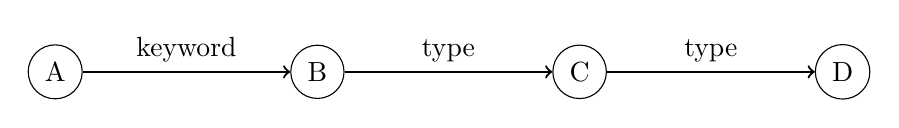
\begin{tikzpicture}
	\tikzset{vertex/.style = {shape=circle,draw,minimum size=.2em}}
	\tikzset{edge/.style = {->,> = latex'}}
	\node[vertex] (a) at  (0,0) {A};
	\node[vertex] (b) at  (3.33,0) {B};
	\node[vertex] (c) at  (6.66,0) {C};
	\node[vertex] (d) at  (10,0) {D};
	\path[->,draw,thick] (a) edge node[above] {keyword} (b);
	\path[->,draw,thick] (b) edge node[above] {type} (c);
	\path[->,draw,thick] (c) edge node[above] {type} (d);
\end{tikzpicture}
\caption{Diagramm einer Methode mit zwei Argumenten}
\label{FIG:DiagramMethodTwoArguments}
\end{figure}

Mehrere Kombinationen von Argumenten werden ebenfalls nicht unterstützt, wenn nur die Typen in der EBNF in einer Alternative vorkommen. Will man eine Methode mit verschiedenen Argumenten überladen, muss man bisher (wie in Listing~\ref{LST:EXPRBNF}) den Namen der Methode und Typ zusammen in alternativen zusammenfassen. Ein solches Konstrukt könnte auf einen Graphen wie in Abbildung~\ref{FIG:DiagramMethodTwoCombinationsArguments} abgebildet werden.
\begin{figure}[ht]
\centering
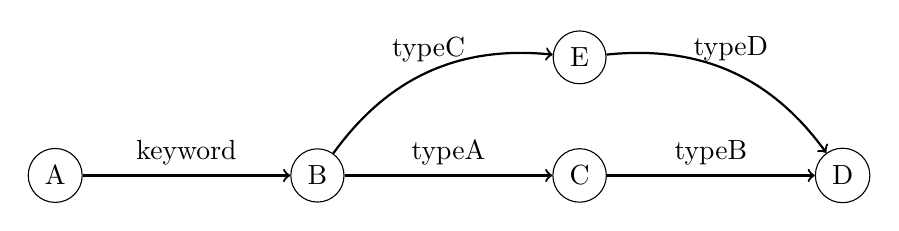
\begin{tikzpicture}
	\tikzset{vertex/.style = {shape=circle,draw,minimum size=.2em}}
	\tikzset{edge/.style = {->,> = latex'}}
	\node[vertex] (a) at  (0,0) {A};
	\node[vertex] (b) at  (3.33,0) {B};
	\node[vertex] (c) at  (6.66,0) {C};
	\node[vertex] (d) at  (10,0) {D};
	\node[vertex] (e) at  (6.66,1.5) {E};
	\path[->,draw,thick] (a) edge node[above] {keyword} (b);
	\path[->,draw,thick] (b) edge node[above] {typeA} (c);
	\path[->,draw,thick] (c) edge node[above] {typeB} (d);
	\path[->,draw,thick, bend left] (b) edge node[above] {typeC} (e);
	\path[->,draw,thick, bend left] (e) edge node[above] {typeD} (d);
\end{tikzpicture}
\caption{Diagramm einer Methode mit zwei verschiedenen Kombinationen von Argumenten}
\label{FIG:DiagramMethodTwoCombinationsArguments}
\end{figure}


\subsection{Unterstützung für Scala-spezifische Konstrukte}
\subsubsection{Operator-Überladung}
\subsubsection{Klammerung und Punkte}
\subsubsection{Implizite und explizite Typumwandlung}


\end{document}
